\documentclass[journal,12pt,onecolumn]{IEEEtran}
\usepackage{amsmath}
\usepackage{multicol}
\usepackage{enumerate}
\usepackage{amssymb}
\usepackage{graphicx}
\usepackage{hyperref}

\begin{document}
\providecommand{\nCr}[2]{\,^{#1}C_{#2}} % nCr
\providecommand{\nPr}[2]{\,^{#1}P_{#2}} % nPr
\providecommand{\mbf}{\mathbf}
\providecommand{\pr}[1]{\ensuremath{\Pr\left(#1\right)}}
\providecommand{\qfunc}[1]{\ensuremath{Q\left(#1\right)}}
\providecommand{\sbrak}[1]{\ensuremath{{}\left[#1\right]}}
\providecommand{\lsbrak}[1]{\ensuremath{{}\left[#1\right.}}
\providecommand{\rsbrak}[1]{\ensuremath{{}\left.#1\right]}}
\providecommand{\brak}[1]{\ensuremath{\left(#1\right)}}
\providecommand{\lbrak}[1]{\ensuremath{\left(#1\right.}}
\providecommand{\rbrak}[1]{\ensuremath{\left.#1\right)}}
\providecommand{\cbrak}[1]{\ensuremath{\left\{#1\right\}}}
\providecommand{\lcbrak}[1]{\ensuremath{\left\{#1\right.}}
\providecommand{\rcbrak}[1]{\ensuremath{\left.#1\right\}}}
\newcommand{\sgn}{\mathop{\mathrm{sgn}}}
\providecommand{\abs}[1]{\left\vert#1\right\vert}
\providecommand{\res}[1]{\Res\displaylimits_{#1}} 
\providecommand{\norm}[1]{\lVert#1\rVert}
\providecommand{\mtx}[1]{\mathbf{#1}}
\providecommand{\mean}[1]{E\left[ #1 \right]}
\providecommand{\fourier}{\overset{\mathcal{F}}{ \rightleftharpoons}}
\providecommand{\hilbert}{\overset{\mathcal{H}}{ \rightleftharpoons}}
\providecommand{\system}{\overset{\mathcal{H}}{ \longleftrightarrow}}

\newcommand{\solution}{\noindent \textbf{Solution: }}
\providecommand{\dec}[2]{\ensuremath{\overset{#1}{\underset{#2}{\gtrless}}}}
\title{ 
Manufacturing Problem
}
\author{Vivek~Srivastava$^{\dagger}$ %<-this  stops a space
\thanks{$\dagger$ The author is with the Department of Electrical Engineering, IIT Hyderabad
502285 India e-mail: ee19mtech11023@iith.ac.in. }
}
\maketitle
\section{Problem Statement}
\begin{enumerate}
 
\item A manufacturing company makes two models A and B of a product. Each piece of Model A requires 9 labour hours for fabricating and 1 labour hour for finishing. Each piece of Model B requires 12 labour hours for fabricating and 3 labour hours for finishing. For fabricating and finishing, the maximum labour hours available are 180 and 30 respectively. The company makes a profit of Rs 8000 on each piece of model A and Rs 12000 on each piece of Model B. How many pieces of Model A and Model B should be manufactured per week to realise a maximum profit? What is the maximum profit per week?
\maketitle
\section{Solution}
Formulation of problem\\

Let,\\ x = number of pieces of model A\\
 y = number of pieces of model B\\
%%and total units transported from Factory P to Depot C will be 8-(x+y) \\as total production capacity of factory P is 8
\\\\
According to the question, the problem can be formulated as:
%%\begin{equation}
%%x+y\leq 8
%%\end{equation}
%%and 
%%\begin{equation}
%%-x-y\leq -4
%%\end{equation}\\
%%Also,\\ number of units transported from Factory Q to depot A is 5-x\\
%%and number of units transported from Factory Q to depot B is 5-y.\\
\\\\
%%The cost function can be written as, 
%%Cost = 10x-70y+1900

\begin{equation}
minimize\hspace{1cm}
\begin{bmatrix}
80000&12000
\end{bmatrix}
\begin{bmatrix}
x\\y
\end{bmatrix}
\end{equation}

subject to
\begin{equation}
\begin{bmatrix}
3&&4\\1&&3
\end{bmatrix}
\begin{bmatrix}
x\\y
\end{bmatrix}
\leq
\begin{bmatrix}
60\\30
\end{bmatrix}
\end{equation}


Fig 1 shows the intersection of various lines and the optimal point indicated as P.
\begin{figure}[h]
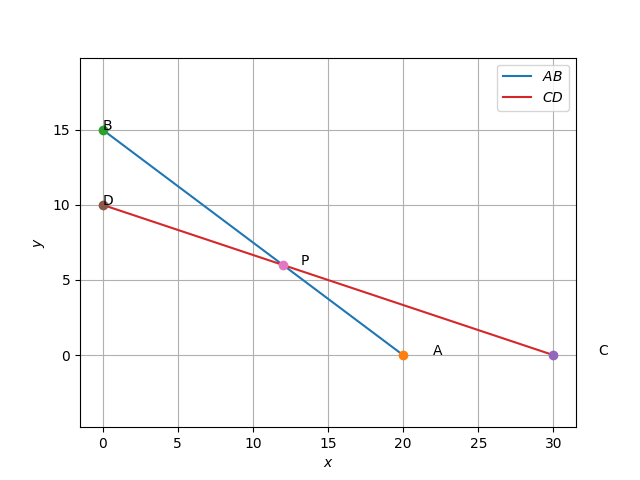
\includegraphics[width=0.9\columnwidth]{Manufacturing.png}
\caption{Solution of Manufacturing Problem}
\end{figure}


\href{https://github.com/vivek13s08/Optimization/blob/master/Manufacturing.py}{Code for generating above image is available here}

\end{enumerate}
\end{document}



